        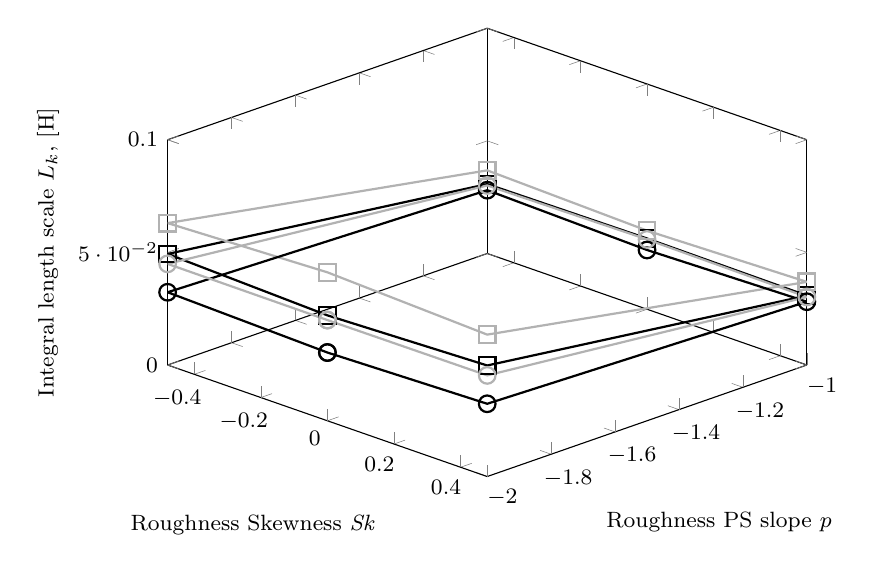
\begin{tikzpicture}[]
        \centering
        \begin{axis}[
        view={45}{35},
            ylabel={Roughness PS slope $p$},
            xlabel={Roughness Skewness \textit{Sk}},
			zlabel={Integral length scale $L_k$, [H]},
			%ztick={5.5,6,6.5,7,7.5},
			zmin=0,zmax=0.1,
            %ymin=0, ymax=0.16,
            width=.8\textwidth,
            height=.6\textwidth,
            label style={font=\footnotesize},
            tick label style={font=\footnotesize}
            ]
                        \addplot3 [
            black,mark=square,thick, mark size=3pt
            ]
            coordinates{
            (0,-2,0.0468)			
			(0.48,-2,0.0493)
			(0.48,-1,0.0308)
			(0,-1,0.0314)
			(-0.48,-1,0.0308)
			(-0.48,-2,0.0493)
            (0,-2,0.0468)
			};
			\addplot3 [
            gray!60,mark=square,thick, mark size=3pt
            ]
            coordinates{
            
            (0,-2,0.0659)
			(0.48,-2,0.0630)
			(0.48,-1,0.0369)
			(0,-1,0.0349)
			(-0.48,-1,0.0369)
			(-0.48,-2,0.0630)
			(0,-2,0.0659)
            };
            
                                    \addplot3 [
            black,mark=o,thick, mark size=3pt
            ]
            coordinates{
            (0,-2,0.0303)			
			(0.48,-2,0.0323)
			(0.48,-1,0.0281)
			(0,-1,0.0263)
			(-0.48,-1,0.0281)
			(-0.48,-2,0.0323)
            (0,-2,0.0303)
			};
			
			
			\addplot3 [
            gray!60,mark=o,thick, mark size=3pt
            ]
            coordinates{
            
            (0,-2,0.0447)
			(0.48,-2,0.0449)
			(0.48,-1,0.0302)
			(0,-1,0.0310)
			(-0.48,-1,0.0302)
			(-0.48,-2,0.0449)
			(0,-2,0.0447)
            };
            
            
            
            
            
        \end{axis}
        \end{tikzpicture}